% Figure 1 of the paper: workflow of the study. Compile standalone (TeX Live with tgheros, sfmath and TikZ):
%   pdflatex -output-directory outputs/figures analysis/fig1_workflow.tex
\documentclass[border=3pt]{standalone}
\usepackage[T1]{fontenc}
\usepackage{tgheros}
\renewcommand*\familydefault{\sfdefault}
\usepackage{amsmath}
\usepackage{sfmath}
\usepackage{tikz}
\usetikzlibrary{arrows.meta, positioning, fit, backgrounds, calc}
\begin{document}
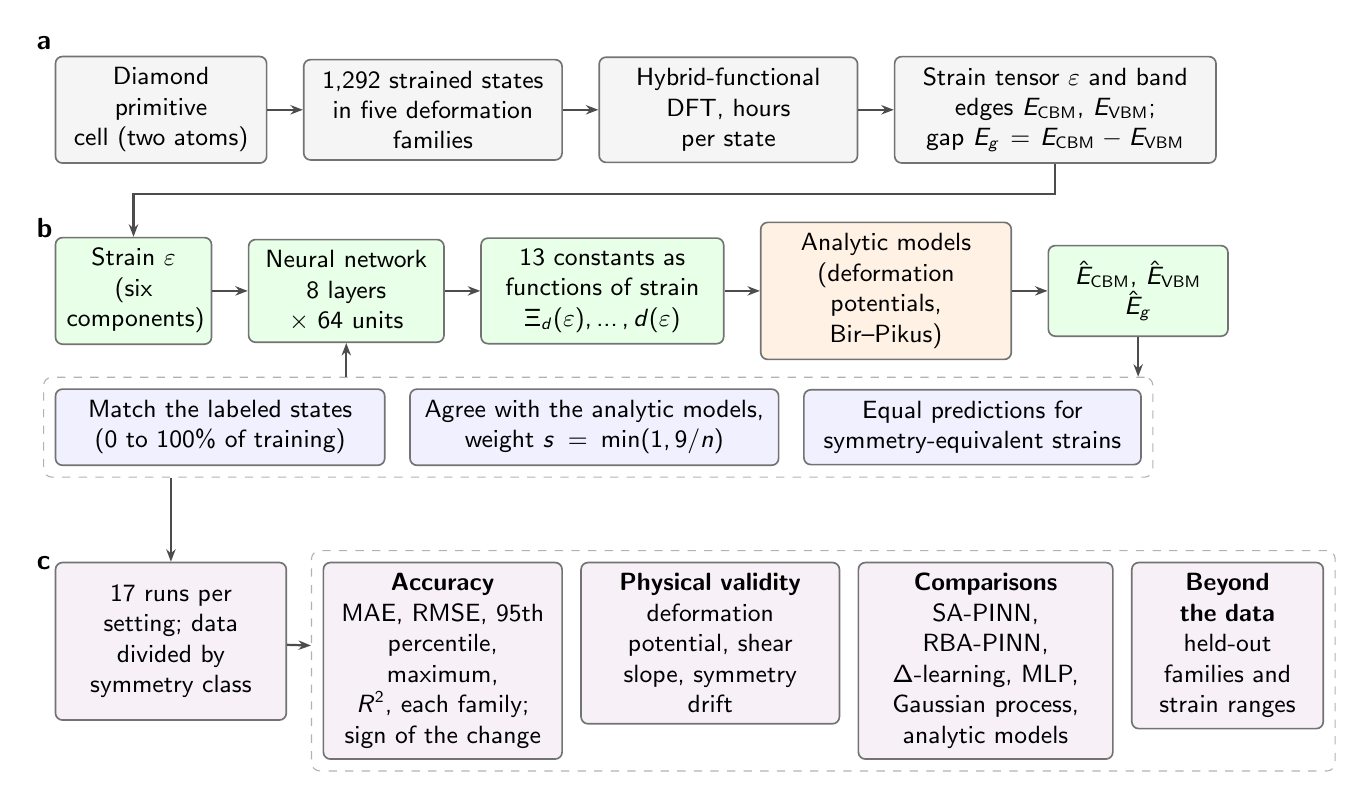
\begin{tikzpicture}[
  font=\sffamily\small,
  box/.style={rectangle, rounded corners=2.5pt, draw=black!55, line width=0.6pt, align=center, inner sep=4pt, minimum height=1.15cm},
  ref/.style={box, fill=black!4},
  net/.style={box, fill=green!9},
  phys/.style={box, fill=orange!10},
  obj/.style={box, fill=blue!6, minimum height=0.95cm},
  ev/.style={box, fill=violet!6},
  ar/.style={-{Stealth[length=4.5pt]}, black!70, line width=0.8pt},
  pl/.style={font=\sffamily\normalsize\bfseries, anchor=north west},
]
%-------------------------------------------------------------- a: reference calculations
\node[pl] at (-0.35, 1.05) {a};
\node[ref, anchor=west, text width=2.4cm] (a1) at (0, 0) {Diamond primitive\\cell (two atoms)};
\node[ref, anchor=west, text width=3.0cm] (a2) at ([xshift=0.45cm]a1.east) {1{,}292 strained states\\in five deformation\\families};
\node[ref, anchor=west, text width=3.0cm] (a3) at ([xshift=0.45cm]a2.east) {Hybrid-functional\\DFT, hours\\per state};
\node[ref, anchor=west, text width=3.8cm] (a4) at ([xshift=0.45cm]a3.east) {Strain tensor $\varepsilon$ and band\\edges $E_{\mathrm{CBM}}$, $E_{\mathrm{VBM}}$;\\gap $E_g = E_{\mathrm{CBM}} - E_{\mathrm{VBM}}$};
\draw[ar] (a1) -- (a2); \draw[ar] (a2) -- (a3); \draw[ar] (a3) -- (a4);
%-------------------------------------------------------------- b: our model
\node[pl] at (-0.35, -1.25) {b};
\node[net, anchor=west, text width=1.7cm] (b1) at (0, -2.3) {Strain $\varepsilon$\\(six\\components)};
\node[net, anchor=west, text width=2.2cm] (b2) at ([xshift=0.45cm]b1.east) {Neural network\\8 layers\\$\times$ 64 units};
\node[net, anchor=west, text width=2.8cm] (b3) at ([xshift=0.45cm]b2.east) {13 constants as\\functions of strain\\$\Xi_d(\varepsilon), \ldots, d(\varepsilon)$};
\node[phys, anchor=west, text width=2.9cm] (b4) at ([xshift=0.45cm]b3.east) {Analytic models\\(deformation potentials,\\Bir--Pikus)};
\node[net, anchor=west, text width=2.0cm] (b5) at ([xshift=0.45cm]b4.east) {$\hat{E}_{\mathrm{CBM}}$, $\hat{E}_{\mathrm{VBM}}$\\$\hat{E}_g$};
\draw[ar] (b1) -- (b2); \draw[ar] (b2) -- (b3); \draw[ar] (b3) -- (b4); \draw[ar] (b4) -- (b5);
\node[obj, anchor=north west, text width=3.9cm] (o1) at ([yshift=-0.55cm]b1.south west) {Match the labeled states\\(0 to 100\% of training)};
\node[obj, anchor=west, text width=4.4cm] (o2) at ([xshift=0.3cm]o1.east) {Agree with the analytic models,\\weight $s = \min(1, 9/n)$};
\node[obj, anchor=west, text width=4.0cm] (o3) at ([xshift=0.3cm]o2.east) {Equal predictions for\\symmetry-equivalent strains};

\begin{scope}[on background layer]
  \node[draw=black!30, dashed, rounded corners=3pt, inner sep=4pt, fit=(o1)(o2)(o3)] (obj) {};
\end{scope}
\draw[ar] (obj.north -| b2.south) -- (b2.south);
\draw[ar] (b5.south) -- (b5.south |- obj.north);
\draw[ar] (a4.south) -- ++(0,-0.38) -| (b1.north);
%-------------------------------------------------------------- c: evaluation
\node[pl] at (-0.35, -5.55) {c};
\node[ev, anchor=west, text width=2.65cm, minimum height=2.0cm] (c1) at (0, -6.75) {17 runs per\\setting; data\\divided by\\symmetry class};
\node[ev, anchor=north west, text width=2.75cm, minimum height=2.0cm] (c2) at ([xshift=0.45cm]c1.north east) {\textbf{Accuracy}\\MAE, RMSE, 95th\\percentile, maximum,\\$R^2$, each family;\\sign of the change};
\node[ev, anchor=north west, text width=3.0cm, minimum height=2.0cm] (c3) at ([xshift=0.22cm]c2.north east) {\textbf{Physical validity}\\deformation\\potential, shear\\slope, symmetry\\drift};
\node[ev, anchor=north west, text width=2.95cm, minimum height=2.0cm] (c4) at ([xshift=0.22cm]c3.north east) {\textbf{Comparisons}\\SA-PINN, RBA-PINN,\\$\Delta$-learning, MLP,\\Gaussian process,\\analytic models};
\node[ev, anchor=north west, text width=2.15cm, minimum height=2.0cm] (c5) at ([xshift=0.22cm]c4.north east) {\textbf{Beyond the data}\\held-out\\families and\\strain ranges};
\begin{scope}[on background layer]
  \node[draw=black!30, dashed, rounded corners=3pt, inner sep=4pt, fit=(c2)(c3)(c4)(c5)] (cg) {};
\end{scope}
\draw[ar] (c1) -- (cg);
\draw[ar] (obj.south -| c1.north) -- (c1.north);
\end{tikzpicture}
\end{document}
